\documentclass{standalone}
\usepackage{tikz}
\usetikzlibrary{patterns, positioning}


\begin{document}
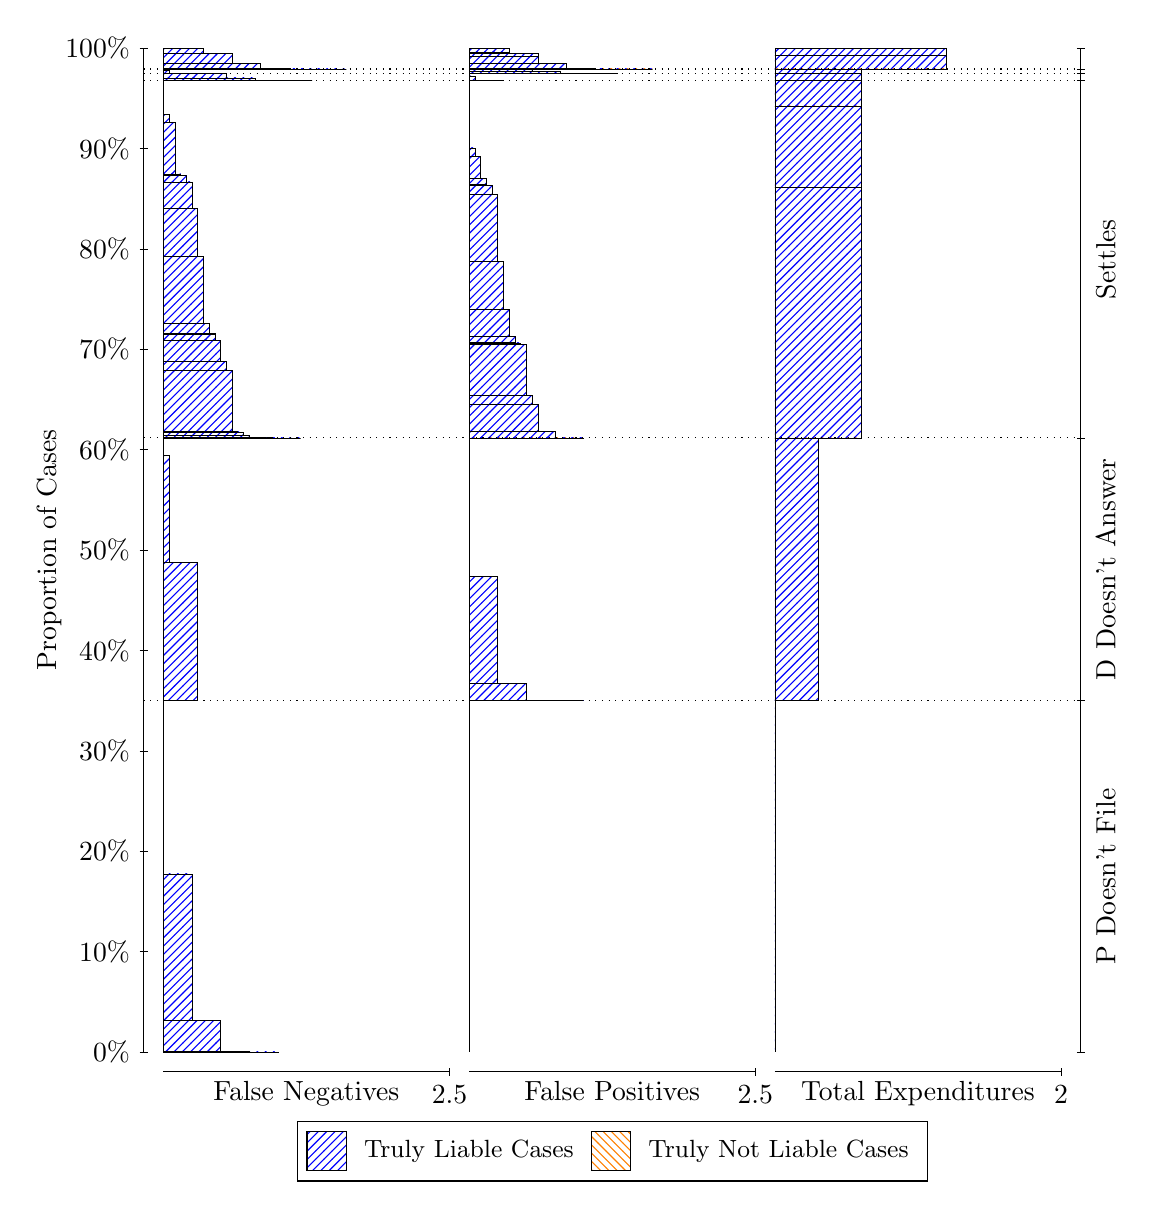
\begin{tikzpicture}
\draw[black, very thin] (1.5,1.75) -- (1.5,14.5);
\node[rotate=90, text=black, anchor=center] at (0.3, 8.125) {Proportion of Cases};
\draw[black, very thin] (1.45,1.75) -- (1.55,1.75);
\node[text=black, anchor=east] at (1.45, 1.75) {0\%};
\draw[black, very thin] (1.45,3.025) -- (1.55,3.025);
\node[text=black, anchor=east] at (1.45, 3.025) {10\%};
\draw[black, very thin] (1.45,4.3) -- (1.55,4.3);
\node[text=black, anchor=east] at (1.45, 4.3) {20\%};
\draw[black, very thin] (1.45,5.575) -- (1.55,5.575);
\node[text=black, anchor=east] at (1.45, 5.575) {30\%};
\draw[black, very thin] (1.45,6.85) -- (1.55,6.85);
\node[text=black, anchor=east] at (1.45, 6.85) {40\%};
\draw[black, very thin] (1.45,8.125) -- (1.55,8.125);
\node[text=black, anchor=east] at (1.45, 8.125) {50\%};
\draw[black, very thin] (1.45,9.4) -- (1.55,9.4);
\node[text=black, anchor=east] at (1.45, 9.4) {60\%};
\draw[black, very thin] (1.45,10.675) -- (1.55,10.675);
\node[text=black, anchor=east] at (1.45, 10.675) {70\%};
\draw[black, very thin] (1.45,11.95) -- (1.55,11.95);
\node[text=black, anchor=east] at (1.45, 11.95) {80\%};
\draw[black, very thin] (1.45,13.225) -- (1.55,13.225);
\node[text=black, anchor=east] at (1.45, 13.225) {90\%};
\draw[black, very thin] (1.45,14.5) -- (1.55,14.5);
\node[text=black, anchor=east] at (1.45, 14.5) {100\%};

\draw[black, very thin] (13.4,1.75) -- (13.4,14.5);
\draw[black, very thin] (13.35,1.75) -- (13.45,1.75);
\node[anchor=west] at (13.35, 1.75) {};
\draw[black, very thin] (13.35,6.2103) -- (13.45,6.2103);
\node[anchor=west] at (13.35, 6.2103) {};
\draw[black, very thin] (13.35,9.5493) -- (13.45,9.5493);
\node[anchor=west] at (13.35, 9.5493) {};
\draw[black, very thin] (13.35,14.088) -- (13.45,14.088);
\node[anchor=west] at (13.35, 14.088) {};
\draw[black, very thin] (13.35,14.179) -- (13.45,14.179);
\node[anchor=west] at (13.35, 14.179) {};
\draw[black, very thin] (13.35,14.234) -- (13.45,14.234);
\node[anchor=west] at (13.35, 14.234) {};
\draw[black, very thin] (13.35,14.5) -- (13.45,14.5);
\node[anchor=west] at (13.35, 14.5) {};

\draw[black, very thin, pattern color=blue, pattern=north east lines] (1.75,1.75) rectangle (3.2033,1.7501);
\draw[black, very thin, pattern color=blue, pattern=north east lines] (1.75,1.7501) rectangle (2.84,1.762);
\draw[black, very thin, pattern color=blue, pattern=north east lines] (1.75,1.762) rectangle (2.4767,2.1501);
\draw[black, very thin, pattern color=blue, pattern=north east lines] (1.75,2.1501) rectangle (2.1133,4.0114);
\draw[black, very thin, pattern color=orange, pattern=north west lines] (1.75,4.0114) rectangle (1.75,4.0114);
\draw[black, very thin, pattern color=blue, pattern=north east lines] (1.75,4.0114) rectangle (1.75,6.2103);
\draw[black, very thin, pattern color=blue, pattern=north east lines] (1.75,6.2103) rectangle (2.186,7.9675);
\draw[black, very thin, pattern color=blue, pattern=north east lines] (1.75,7.9675) rectangle (1.8227,9.3258);
\draw[black, very thin, pattern color=orange, pattern=north west lines] (1.75,9.3258) rectangle (1.75,9.3258);
\draw[black, very thin, pattern color=blue, pattern=north east lines] (1.75,9.3258) rectangle (1.75,9.5493);
\draw[black, very thin, pattern color=blue, pattern=north east lines] (1.75,9.5493) rectangle (3.494,9.5493);
\draw[black, very thin, pattern color=blue, pattern=north east lines] (1.75,9.5493) rectangle (3.2033,9.5494);
\draw[black, very thin, pattern color=blue, pattern=north east lines] (1.75,9.5494) rectangle (3.1307,9.5504);
\draw[black, very thin, pattern color=blue, pattern=north east lines] (1.75,9.5504) rectangle (3.058,9.5504);
\draw[black, very thin, pattern color=blue, pattern=north east lines] (1.75,9.5504) rectangle (2.9127,9.5508);
\draw[black, very thin, pattern color=blue, pattern=north east lines] (1.75,9.5508) rectangle (2.84,9.5844);
\draw[black, very thin, pattern color=blue, pattern=north east lines] (1.75,9.5844) rectangle (2.7673,9.6249);
\draw[black, very thin, pattern color=blue, pattern=north east lines] (1.75,9.6249) rectangle (2.6947,9.6306);
\draw[black, very thin, pattern color=blue, pattern=north east lines] (1.75,9.6306) rectangle (2.622,10.406);
\draw[black, very thin, pattern color=blue, pattern=north east lines] (1.75,10.406) rectangle (2.5493,10.519);
\draw[black, very thin, pattern color=blue, pattern=north east lines] (1.75,10.519) rectangle (2.4767,10.794);
\draw[black, very thin, pattern color=blue, pattern=north east lines] (1.75,10.794) rectangle (2.404,10.871);
\draw[black, very thin, pattern color=blue, pattern=north east lines] (1.75,10.871) rectangle (2.404,10.88);
\draw[black, very thin, pattern color=blue, pattern=north east lines] (1.75,10.88) rectangle (2.3313,11.001);
\draw[black, very thin, pattern color=blue, pattern=north east lines] (1.75,11.001) rectangle (2.2587,11.851);
\draw[black, very thin, pattern color=blue, pattern=north east lines] (1.75,11.851) rectangle (2.186,12.459);
\draw[black, very thin, pattern color=blue, pattern=north east lines] (1.75,12.459) rectangle (2.1133,12.8);
\draw[black, very thin, pattern color=blue, pattern=north east lines] (1.75,12.8) rectangle (2.0407,12.881);
\draw[black, very thin, pattern color=blue, pattern=north east lines] (1.75,12.881) rectangle (2.0407,12.881);
\draw[black, very thin, pattern color=blue, pattern=north east lines] (1.75,12.881) rectangle (1.968,12.902);
\draw[black, very thin, pattern color=blue, pattern=north east lines] (1.75,12.902) rectangle (1.8953,13.554);
\draw[black, very thin, pattern color=blue, pattern=north east lines] (1.75,13.554) rectangle (1.8227,13.659);
\draw[black, very thin, pattern color=orange, pattern=north west lines] (1.75,13.659) rectangle (1.75,13.659);
\draw[black, very thin, pattern color=blue, pattern=north east lines] (1.75,13.659) rectangle (1.75,14.088);
\draw[black, very thin, pattern color=blue, pattern=north east lines] (1.75,14.088) rectangle (3.6393,14.088);
\draw[black, very thin, pattern color=blue, pattern=north east lines] (1.75,14.088) rectangle (3.276,14.088);
\draw[black, very thin, pattern color=blue, pattern=north east lines] (1.75,14.088) rectangle (2.9127,14.122);
\draw[black, very thin, pattern color=blue, pattern=north east lines] (1.75,14.122) rectangle (2.5493,14.177);
\draw[black, very thin, pattern color=blue, pattern=north east lines] (1.75,14.177) rectangle (2.186,14.179);
\draw[black, very thin, pattern color=orange, pattern=north west lines] (1.75,14.179) rectangle (1.75,14.179);
\draw[black, very thin, pattern color=blue, pattern=north east lines] (1.75,14.179) rectangle (2.186,14.179);
\draw[black, very thin, pattern color=blue, pattern=north east lines] (1.75,14.179) rectangle (1.8227,14.213);
\draw[black, very thin, pattern color=orange, pattern=north west lines] (1.75,14.213) rectangle (1.75,14.213);
\draw[black, very thin, pattern color=blue, pattern=north east lines] (1.75,14.213) rectangle (1.75,14.234);
\draw[black, very thin, pattern color=blue, pattern=north east lines] (1.75,14.234) rectangle (4.0753,14.234);
\draw[black, very thin, pattern color=blue, pattern=north east lines] (1.75,14.234) rectangle (3.712,14.234);
\draw[black, very thin, pattern color=blue, pattern=north east lines] (1.75,14.234) rectangle (3.3487,14.238);
\draw[black, very thin, pattern color=blue, pattern=north east lines] (1.75,14.238) rectangle (2.9853,14.3);
\draw[black, very thin, pattern color=blue, pattern=north east lines] (1.75,14.3) rectangle (2.622,14.434);
\draw[black, very thin, pattern color=blue, pattern=north east lines] (1.75,14.434) rectangle (2.2587,14.495);
\draw[black, very thin, pattern color=blue, pattern=north east lines] (1.75,14.495) rectangle (1.8953,14.5);
\draw[black, very thin, pattern color=orange, pattern=north west lines] (1.75,14.5) rectangle (1.75,14.5);
\draw[black, very thin, pattern color=blue, pattern=north east lines] (1.75,14.5) rectangle (1.75,14.5);
\draw[black, very thin, pattern color=orange, pattern=north west lines] (5.6333,1.75) rectangle (5.6333,1.75);
\draw[black, very thin, pattern color=blue, pattern=north east lines] (5.6333,1.75) rectangle (5.6333,6.2103);
\draw[black, very thin, pattern color=orange, pattern=north west lines] (5.6333,6.2103) rectangle (7.0867,6.2103);
\draw[black, very thin, pattern color=blue, pattern=north east lines] (5.6333,6.2103) rectangle (7.0867,6.2103);
\draw[black, very thin, pattern color=blue, pattern=north east lines] (5.6333,6.2103) rectangle (6.7233,6.2113);
\draw[black, very thin, pattern color=blue, pattern=north east lines] (5.6333,6.2113) rectangle (6.36,6.4337);
\draw[black, very thin, pattern color=blue, pattern=north east lines] (5.6333,6.4337) rectangle (5.9967,7.7921);
\draw[black, very thin, pattern color=blue, pattern=north east lines] (5.6333,7.7921) rectangle (5.6333,9.5493);
\draw[black, very thin, pattern color=orange, pattern=north west lines] (5.6333,9.5493) rectangle (7.0867,9.5493);
\draw[black, very thin, pattern color=blue, pattern=north east lines] (5.6333,9.5493) rectangle (7.0867,9.5495);
\draw[black, very thin, pattern color=orange, pattern=north west lines] (5.6333,9.5495) rectangle (6.9413,9.5495);
\draw[black, very thin, pattern color=blue, pattern=north east lines] (5.6333,9.5495) rectangle (6.9413,9.5495);
\draw[black, very thin, pattern color=orange, pattern=north west lines] (5.6333,9.5495) rectangle (6.796,9.5495);
\draw[black, very thin, pattern color=blue, pattern=north east lines] (5.6333,9.5495) rectangle (6.796,9.5498);
\draw[black, very thin, pattern color=blue, pattern=north east lines] (5.6333,9.5498) rectangle (6.7233,9.6283);
\draw[black, very thin, pattern color=orange, pattern=north west lines] (5.6333,9.6283) rectangle (6.6507,9.6283);
\draw[black, very thin, pattern color=blue, pattern=north east lines] (5.6333,9.6283) rectangle (6.6507,9.6285);
\draw[black, very thin, pattern color=blue, pattern=north east lines] (5.6333,9.6285) rectangle (6.578,9.6314);
\draw[black, very thin, pattern color=orange, pattern=north west lines] (5.6333,9.6314) rectangle (6.5053,9.6314);
\draw[black, very thin, pattern color=blue, pattern=north east lines] (5.6333,9.6314) rectangle (6.5053,9.9789);
\draw[black, very thin, pattern color=blue, pattern=north east lines] (5.6333,9.9789) rectangle (6.4327,10.084);
\draw[black, very thin, pattern color=blue, pattern=north east lines] (5.6333,10.084) rectangle (6.36,10.735);
\draw[black, very thin, pattern color=blue, pattern=north east lines] (5.6333,10.735) rectangle (6.2873,10.756);
\draw[black, very thin, pattern color=orange, pattern=north west lines] (5.6333,10.756) rectangle (6.2147,10.756);
\draw[black, very thin, pattern color=blue, pattern=north east lines] (5.6333,10.756) rectangle (6.2147,10.757);
\draw[black, very thin, pattern color=blue, pattern=north east lines] (5.6333,10.757) rectangle (6.2147,10.838);
\draw[black, very thin, pattern color=blue, pattern=north east lines] (5.6333,10.838) rectangle (6.142,11.178);
\draw[black, very thin, pattern color=blue, pattern=north east lines] (5.6333,11.178) rectangle (6.0693,11.787);
\draw[black, very thin, pattern color=blue, pattern=north east lines] (5.6333,11.787) rectangle (5.9967,12.637);
\draw[black, very thin, pattern color=blue, pattern=north east lines] (5.6333,12.637) rectangle (5.924,12.758);
\draw[black, very thin, pattern color=blue, pattern=north east lines] (5.6333,12.758) rectangle (5.8513,12.767);
\draw[black, very thin, pattern color=blue, pattern=north east lines] (5.6333,12.767) rectangle (5.8513,12.844);
\draw[black, very thin, pattern color=blue, pattern=north east lines] (5.6333,12.844) rectangle (5.7787,13.119);
\draw[black, very thin, pattern color=blue, pattern=north east lines] (5.6333,13.119) rectangle (5.706,13.232);
\draw[black, very thin, pattern color=blue, pattern=north east lines] (5.6333,13.232) rectangle (5.6333,14.088);
\draw[black, very thin, pattern color=orange, pattern=north west lines] (5.6333,14.088) rectangle (6.0693,14.088);
\draw[black, very thin, pattern color=blue, pattern=north east lines] (5.6333,14.088) rectangle (6.0693,14.09);
\draw[black, very thin, pattern color=blue, pattern=north east lines] (5.6333,14.09) rectangle (5.706,14.145);
\draw[black, very thin, pattern color=blue, pattern=north east lines] (5.6333,14.145) rectangle (5.6333,14.179);
\draw[black, very thin, pattern color=orange, pattern=north west lines] (5.6333,14.179) rectangle (7.5227,14.179);
\draw[black, very thin, pattern color=blue, pattern=north east lines] (5.6333,14.179) rectangle (7.5227,14.179);
\draw[black, very thin, pattern color=blue, pattern=north east lines] (5.6333,14.179) rectangle (7.1593,14.179);
\draw[black, very thin, pattern color=blue, pattern=north east lines] (5.6333,14.179) rectangle (6.796,14.199);
\draw[black, very thin, pattern color=blue, pattern=north east lines] (5.6333,14.199) rectangle (6.4327,14.233);
\draw[black, very thin, pattern color=blue, pattern=north east lines] (5.6333,14.233) rectangle (6.0693,14.234);
\draw[black, very thin, pattern color=orange, pattern=north west lines] (5.6333,14.234) rectangle (7.9587,14.234);
\draw[black, very thin, pattern color=blue, pattern=north east lines] (5.6333,14.234) rectangle (7.9587,14.234);
\draw[black, very thin, pattern color=orange, pattern=north west lines] (5.6333,14.234) rectangle (7.5953,14.234);
\draw[black, very thin, pattern color=blue, pattern=north east lines] (5.6333,14.234) rectangle (7.5953,14.234);
\draw[black, very thin, pattern color=orange, pattern=north west lines] (5.6333,14.234) rectangle (7.232,14.234);
\draw[black, very thin, pattern color=blue, pattern=north east lines] (5.6333,14.234) rectangle (7.232,14.239);
\draw[black, very thin, pattern color=blue, pattern=north east lines] (5.6333,14.239) rectangle (6.8687,14.3);
\draw[black, very thin, pattern color=orange, pattern=north west lines] (5.6333,14.3) rectangle (6.8687,14.3);
\draw[black, very thin, pattern color=blue, pattern=north east lines] (5.6333,14.3) rectangle (6.8687,14.3);
\draw[black, very thin, pattern color=blue, pattern=north east lines] (5.6333,14.3) rectangle (6.5053,14.395);
\draw[black, very thin, pattern color=orange, pattern=north west lines] (5.6333,14.395) rectangle (6.5053,14.395);
\draw[black, very thin, pattern color=blue, pattern=north east lines] (5.6333,14.395) rectangle (6.5053,14.434);
\draw[black, very thin, pattern color=blue, pattern=north east lines] (5.6333,14.434) rectangle (6.142,14.45);
\draw[black, very thin, pattern color=blue, pattern=north east lines] (5.6333,14.45) rectangle (6.142,14.496);
\draw[black, very thin, pattern color=blue, pattern=north east lines] (5.6333,14.496) rectangle (5.7787,14.496);
\draw[black, very thin, pattern color=blue, pattern=north east lines] (5.6333,14.496) rectangle (5.7787,14.5);
\draw[black, very thin, pattern color=blue, pattern=north east lines] (5.6333,14.5) rectangle (5.6333,14.5);
\draw[black, very thin, pattern color=orange, pattern=north west lines] (9.5167,1.75) rectangle (9.5167,1.75);
\draw[black, very thin, pattern color=blue, pattern=north east lines] (9.5167,1.75) rectangle (9.5167,6.2103);
\draw[black, very thin, pattern color=orange, pattern=north west lines] (9.5167,6.2103) rectangle (10.062,6.2103);
\draw[black, very thin, pattern color=blue, pattern=north east lines] (9.5167,6.2103) rectangle (10.062,9.5493);
\draw[black, very thin, pattern color=orange, pattern=north west lines] (9.5167,9.5493) rectangle (10.607,9.5493);
\draw[black, very thin, pattern color=blue, pattern=north east lines] (9.5167,9.5493) rectangle (10.607,12.732);
\draw[black, very thin, pattern color=orange, pattern=north west lines] (9.5167,12.732) rectangle (10.607,12.732);
\draw[black, very thin, pattern color=blue, pattern=north east lines] (9.5167,12.732) rectangle (10.607,13.765);
\draw[black, very thin, pattern color=orange, pattern=north west lines] (9.5167,13.765) rectangle (10.607,13.765);
\draw[black, very thin, pattern color=blue, pattern=north east lines] (9.5167,13.765) rectangle (10.607,14.088);
\draw[black, very thin, pattern color=orange, pattern=north west lines] (9.5167,14.088) rectangle (10.607,14.088);
\draw[black, very thin, pattern color=blue, pattern=north east lines] (9.5167,14.088) rectangle (10.607,14.179);
\draw[black, very thin, pattern color=orange, pattern=north west lines] (9.5167,14.179) rectangle (10.607,14.179);
\draw[black, very thin, pattern color=blue, pattern=north east lines] (9.5167,14.179) rectangle (10.607,14.234);
\draw[black, very thin, pattern color=orange, pattern=north west lines] (9.5167,14.234) rectangle (11.697,14.234);
\draw[black, very thin, pattern color=blue, pattern=north east lines] (9.5167,14.234) rectangle (11.697,14.41);
\draw[black, very thin, pattern color=orange, pattern=north west lines] (9.5167,14.41) rectangle (11.697,14.41);
\draw[black, very thin, pattern color=blue, pattern=north east lines] (9.5167,14.41) rectangle (11.697,14.5);
\draw[black, dotted] (1.5,6.2103) -- (13.4,6.2103);
\draw[black, dotted] (1.5,9.5493) -- (13.4,9.5493);
\draw[black, dotted] (1.5,14.088) -- (13.4,14.088);
\draw[black, dotted] (1.5,14.179) -- (13.4,14.179);
\draw[black, dotted] (1.5,14.234) -- (13.4,14.234);
\draw[black, very thin] (1.75,1.5) -- (5.3833,1.5);
\node[text=black, anchor=north] at (3.5667, 1.5) {False Negatives};
\draw[black, very thin] (5.3833,1.45) -- (5.3833,1.55);
\node[text=black, anchor=north] at (5.3833, 1.45) {2.5};

\draw[black, very thin] (5.6333,1.5) -- (9.2667,1.5);
\node[text=black, anchor=north] at (7.45, 1.5) {False Positives};
\draw[black, very thin] (9.2667,1.45) -- (9.2667,1.55);
\node[text=black, anchor=north] at (9.2667, 1.45) {2.5};

\draw[black, very thin] (9.5167,1.5) -- (13.15,1.5);
\node[text=black, anchor=north] at (11.333, 1.5) {Total Expenditures};
\draw[black, very thin] (13.15,1.45) -- (13.15,1.55);
\node[text=black, anchor=north] at (13.15, 1.45) {2};

\node[text=black, centered, rotate=90] at (13.72, 3.9801) {P Doesn't File};
\node[text=black, centered, rotate=90] at (13.72, 7.8798) {D Doesn't Answer};
\node[text=black, centered, rotate=90] at (13.72, 11.819) {Settles};




\draw (7.449999999999999,1.5) node[draw=none] (baseCoordinate) {};
\begin{scope}[align=center]
        \matrix[scale=0.5, draw=black, below=0.5cm of baseCoordinate, nodes={draw}, column sep=0.1cm]{
            \node[rectangle, draw, minimum width=0.5cm, minimum height=0.5cm, pattern color=blue, pattern=north east lines] {}; &
            \node[draw=none, font=\small, text=black] (B) {Truly Liable Cases}; &
            \node[rectangle, draw, minimum width=0.5cm, minimum height=0.5cm, pattern color=orange, pattern=north west lines] {}; &
            \node[draw=none, font=\small, text=black] (B) {Truly Not Liable Cases}; \\
            };
\end{scope}

\end{tikzpicture}
\end{document}